\section{Qu'est-ce qu'un labyrinthe ?}
\subsection{Définition d'un labyrinthe}
Un labyrinthe est une structure complexe de passages reliés entre-eux. L’objectif du solveur est de passer d'un point de départ à un point d'arrivée, c'est-à-dire trouver le passage reliant ces deux points. Le labyrinthe est une énigme qui teste l'intelligence, la réflexion, et la rapidité d'exécutions du solveur. D'un point de vu mathématique, les labyrinthes peuvent êtres représentés comme étant des surfaces connexes. 


\subsection{Histoire et application}
Le mot labyrinthe trouve son origine dans la  mythologie grecque, c'était une structure constitué de galeries, construite par Dédale afin d'y enfermer le Minotaure.
Le divertissement et l'entraînement cérébral peuvent être considérés comme les principaux objectifs d'application d'un labyrinthe.
En ce qui concerne le domaine scientifique, les labyrinthes peuvent être vu comme des supports pour effectuer des démonstrations robotiques. Le concept de labyrinthe a permis la naissance de concours robotiques comme les compétitions Micromouses ou l'objectif est de résoudre une énigme (un labyrinthe) en ayant recours à différents algorithmes d'intelligence artificielle.
\section{Classification d'un labyrinthe} 
\label{sec:ProblematiqueConstructionLabyrinthe}
\paragraph{}
Les labyrinthes (et les algorithmes responsables de leur génération) peuvent être organisés selon trois critères de  classifications différents. Ces critères sont : la dimension, la topologie, et la tessellation. Un labyrinthe peut prendre un objet d'un de ses classes dans n'importe quelle combinaison.

\subsection{Dimension d'un labyrinthe}
La dimension d'un labyrinthe corresponds à l'espace dimensionnel couvert par le labyrinthe. Les labyrinthes peuvent êtres de dimensionnalité 2, 3 ou tout autre dimension supérieure.

\begin{figure*}[htp] 
    \centering
    \subfloat[Labyrinthe en 2 dimensions.]{%
        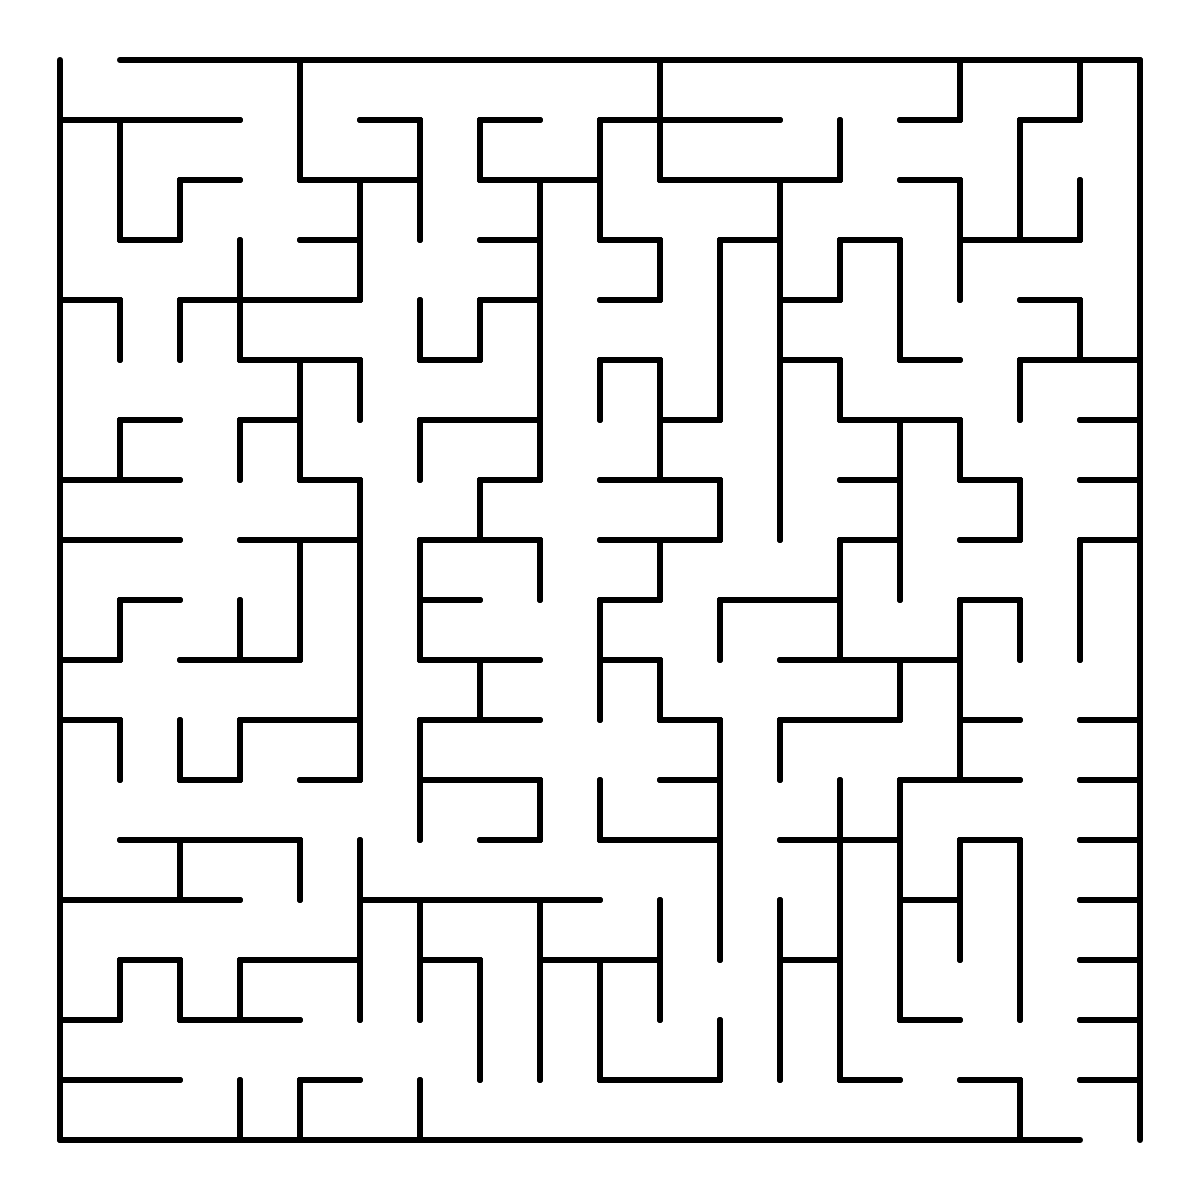
\includegraphics[width=0.35\textwidth]{report/pics/2D_maze.png}%
        \label{fig:a}%
        }%
    \hfill%
    \subfloat[Labyrinthe en 3 dimensions.]{%
        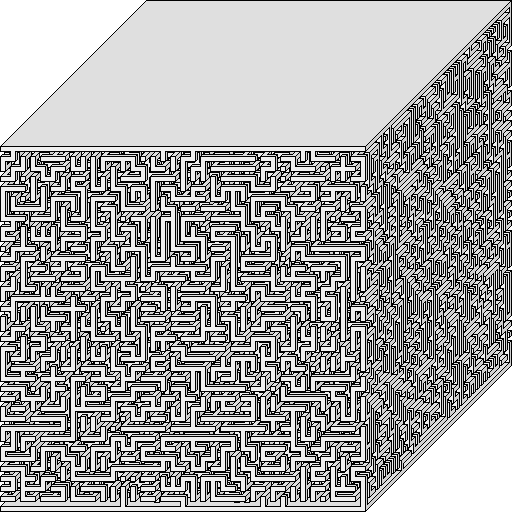
\includegraphics[width=0.35\textwidth]{pics/3D_maze.png}%
        \label{fig:b}%
        }%
    \caption{Exemple d'un labyrinthe 2D et d'un labyrinthe 3D}
\end{figure*}


\subsection{Tessellation d'un labyrinthe}
La classe de tessellation est la géométrie des cellules individuelles qui composent le labyrinthe. Il existe de nombreux types de tessellation, on citera notamment :
\begin{itemize}
\item\textbf{ Tesellation orthogonale :} Il s'agit d'une grille rectangulaire standard où les cellules ont des passages qui se coupent à angle droit formant des cellules sous forme de carrés.

\item\textbf{Tesellation delta :} Un labyrinthe à tessellation delta est un composé de triangles imbriqués, où chaque cellule peut avoir jusqu'à trois passages connectés.

\item\textbf{Tesellation theta :} Un labyrinthe à tessellation theta est composé de cercles concentriques. Les cellules ont généralement quatre connexions de passage possibles, mais peuvent en avoir plus en raison du plus grand nombre de cellules dans les anneaux externes.
\end{itemize}

\begin{figure*}[htp] 
    \centering
    \subfloat[Labyrinthe orthogonal.]{%
        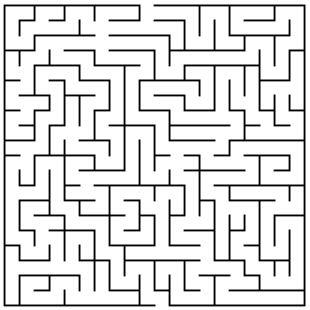
\includegraphics[width=0.27\textwidth]{report/pics/orthogonal_maze.png}%
        \label{fig:a}%
        }%
    \hfill%
    \subfloat[Labyrinthe delta.]{%
        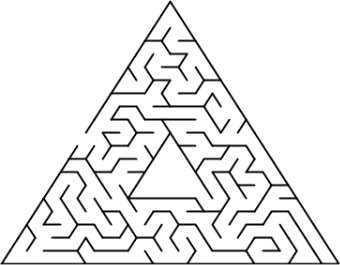
\includegraphics[width=0.3\textwidth]{report/pics/delta_maze.png}%
        \label{fig:b}%
        }%
        \hfill%
    \subfloat[Labyrinthe theta.]{%
        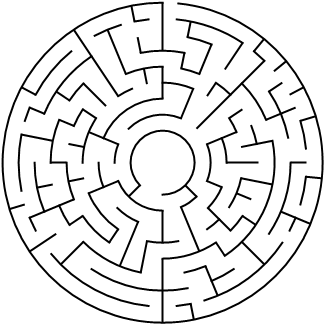
\includegraphics[width=0.3\textwidth]{report/pics/theta_maze.png}%
        \label{fig:c}%
        }%
    \caption{Exemple de labyrinthes avec différentes classes de tessellation.}
\end{figure*}


\subsection{Topologie d'un labyrinthe}
D’un point de vu mathématique, un labyrinthe est définie comme étant une surface connexe pouvant avoir deux types de topologies : topologie simple et topologie comportant des anneaux. Cette différence dans le type de topologie conduit à une distinction des labyrinthes en deux catégories : Les labyrinthes parfaits et les labyrinthes imparfaits.

\subsubsection{Labyrinthe parfait}
Afin qu'un labyrinthe soit labélisé comme étant parfait, ce dernier doit remplir deux conditions :
\begin{itemize}
\item Ne contient pas de cycles.
\item Il existe un unique chemin entre la cellule de départ et la cellule d’arrivée du labyrinthe.
\end{itemize}
Plus généralement, quelque soit deux cellules sélectionnées dans notre labyrinthe, le chemin entre ces deux cellules doit être unique.

\subsubsection{Labyrinthe imparfait}
Un labyrinthe qui ne remplit pas les conditions pour être labélisé comme parfait est dit imparfait. Les labyrinthes imparfaits peuvent donc contenir des boucles, des îlots ou des cellules inaccessibles.


\begin{figure*}[htp] 
    \centering
    \subfloat[Labyrinthe parfait.]{%
        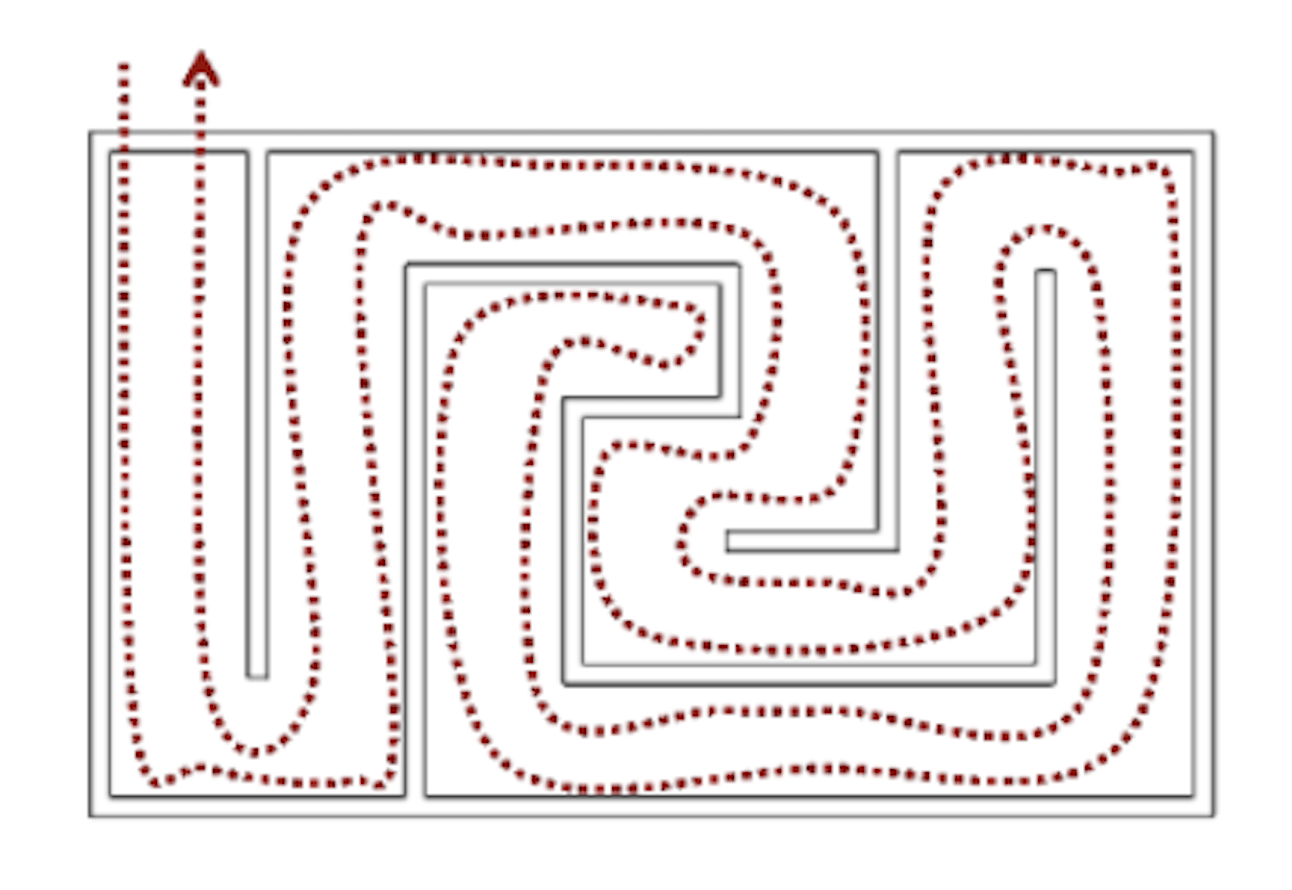
\includegraphics[width=0.5\textwidth]{report/pics/perfect_maze.png}%
        \label{fig:a}%
        }%
    \hfill%
    \subfloat[Labyrinthe imparfait.]{%
        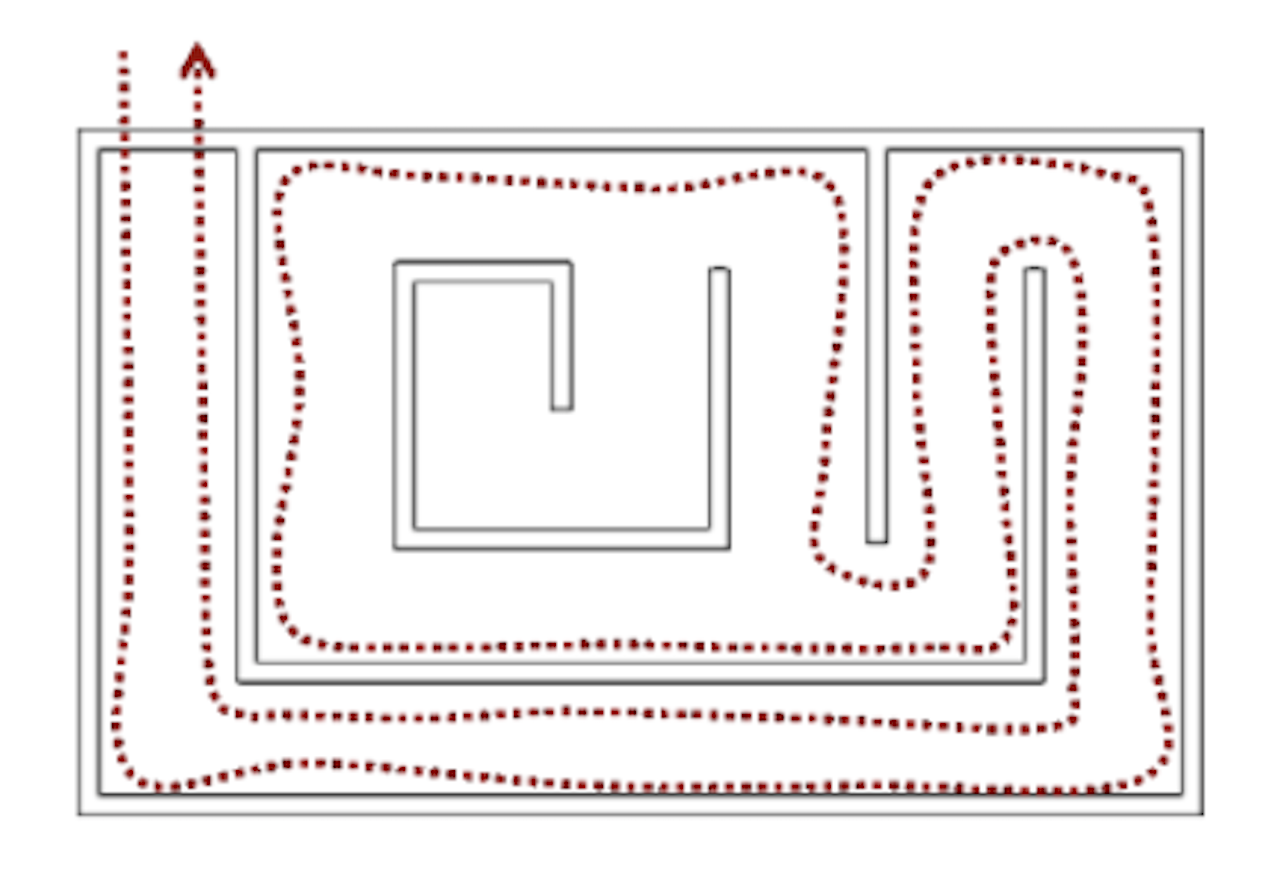
\includegraphics[width=0.5\textwidth]{report/pics/imperfect_maze.png}%
        \label{fig:b}%
        }%
    \caption{Exemple d'un labyrinthe parfait et d'un labyrinthe imparfait.}
\end{figure*}




Dans la suite de ce rapport, nous considérons l'ensemble de nos labyrinthes comme étant de dimension 2 et possédant une tessellation orthogonale. La distinction se feras sur le critère de la topologie, on distinguera alors deux types de labyrinthes : les labyrinthes parfaits et les labyrinthes imparfaits.

\newpage
\section{Introduction à la génération de labyrinthes}
Les algorithmes utilisés pour la génération de labyrinthes suivent un ordre d'étapes prédéfini. Afin de créer des labyrinthes structurés de manière aléatoire, une ou plusieurs étapes de l'algorithme doivent être randomisées (c'est-à-dire que la prise de décision au sein de l'étape doit utiliser une fonction renvoyant un résultat aléatoire). 
Il existe deux approches algorithmiques générales utilisées pour la génération automatisée des labyrinthes. Ces approches sont : l'ajout de murs et la sculpture de passages.
\\
\begin{itemize}
\item\textbf{ Ajout de murs :} Dans cette approche, on se base sur l'ajout de murs pour générer progressivement notre labyrinthe. On démarre d'un labyrinthe vide, puis l'algorithme va placer au fur et à mesure des murs à des positions spécifiques. 
\\
\item\textbf{ Sculpture de passages :} Les algorithmes basés sur cette approche se concentrent sur les chemins et le positionnement des cellules du labyrinthe. On démarre d'une matrice de cellules (une grille complètement remplie de murs), puis l'algorithme de sculpture de passages va alors creuser à travers la grille et détruire certains murs reliant les différentes cellules, ce processus itérative générera au final un labyrinthe.
\end{itemize}
\subsection{Introduction à la théorie des graphes}
Cette sous-section présente certains principes fondamentaux de la théorie des graphes sur lesquels sont basé les algorithmes de génération de labyrinthes. 
\subsubsection{Graphe}
Un graphe est le concept fondamental dans la théorie des graphes, ce dernier est définie comme étant un triplet  $G = (V, E, \epsilon )$, avec $V$ représentant l'ensemble des sommets, $E$  l'ensemble des arêtes et $\epsilon$ une fonction de mappage appelée relation d'incidence tel que $\epsilon$ : $E	\rightarrow \power{V}{2}$

\subsection{Théorie des graphes et génération de labyrinthes}



\section{État de l’art: études des solutions existantes} \label{sec:etatDeLart2}
\subsection{Algorithme de Prim}
\subsection{Algorithme de Kruskal}
\subsection{Algorithme de Backtracking}
\subsection{Algorithme de d'arbre binaire}




\section{Solution proposée et sa mise en œuvre} \label{sec:solution2}
\subsection{Solution implémentée pour la génération de labyrinthes parfaits}
\subsection{Solution implémentée pour la génération de labyrinthes imparfaits}
\paragraph{Chapeau}


\section{Tests et certifications de la solution} \label{sec:test2}

\paragraph{Chapeau}
